% This LaTeX document needs to be compiled with XeLaTeX.
\documentclass[10pt]{article}
\usepackage[utf8]{inputenc}
\usepackage{ucharclasses}
\usepackage{amsmath}
\usepackage{amsfonts}
\usepackage{amssymb}
\usepackage[version=4]{mhchem}
\usepackage{stmaryrd}
\usepackage{graphicx}
\usepackage[export]{adjustbox}
\graphicspath{ {./images/} }
\usepackage{polyglossia}
\usepackage{fontspec}
\setmainlanguage{german}
\setotherlanguages{hindi}
\IfFontExistsTF{Noto Serif Devanagari}
{\newfontfamily\hindifont{Noto Serif Devanagari}}
{\IfFontExistsTF{Kohinoor Devanagari}
  {\newfontfamily\hindifont{Kohinoor Devanagari}}
  {\IfFontExistsTF{Devanagari MT}
    {\newfontfamily\hindifont{Devanagari MT}}
    {\IfFontExistsTF{Lohit Devanagari}
      {\newfontfamily\hindifont{Lohit Devanagari}}
      {\IfFontExistsTF{FreeSerif}
        {\newfontfamily\hindifont{FreeSerif}}
        {\newfontfamily\hindifont{Arial Unicode MS}}
}}}}
\IfFontExistsTF{CMU Serif}
{\newfontfamily\lgcfont{CMU Serif}}
{\IfFontExistsTF{DejaVu Sans}
  {\newfontfamily\lgcfont{DejaVu Sans}}
  {\newfontfamily\lgcfont{Georgia}}
}
\setDefaultTransitions{\lgcfont}{}
\setTransitionsForDevanagari{\hindifont}{\rmfamily}

\title{Hauptprüfung Abiturprüfung 2023 - Leistungsfach }

\author{Alexander Schwarz\\
www.mathe-aufgaben.com}
\date{}


\begin{document}
\maketitle
 Baden-Württemberg

\section*{Aufgabe C1}
Ein Unternehmen stellt Olivenöl her und füllt es in Flaschen ab. Laut Aufdruck beträgt die Füllmenge jeder Flasche 600 ml .\\
Die Flaschen werden in Kartons verpackt; jeder Karton enthält zwölf Flaschen. Ein Karton gilt als fehlerhaft, wenn mehr als eine Flasche weniger als 600 ml Öl enthält. Für jede Flasche beträgt die Wahrscheinlichkeit dafür, dass sie weniger als 600 ml Öl enthält, 1,5\%.\\
a) Die Rechnung $0,985^{12} \approx 83,4 \%$ stellt im Sachzusammenhang die Lösung einer Aufgabe dar. Formulieren Sie eine passende Aufgabenstellung und erläutern Sie den Ansatz der Rechnung.\\
(1,5 VP)\\
b) An einen Supermarkt wird regelmäßig die gleiche Anzahl von Flaschen geliefert. Dabei enthalten im Mittel mehr als 780 Flaschen mindestens 600 ml Öl. Ermitteln Sie, wie viele Flaschen mindestens geliefert werden.\\
c) Ein Supermarkt erhält eine Lieferung von 150 Kartons. Bestimmen Sie die Wahrscheinlichkeit dafür, dass mehr als 3\% der Kartons fehlerhaft sind.\\
(2 VP)\\
Die Füllmenge der Flaschen soll als normalverteilt mit einem Erwartungswert von $600,5 \mathrm{ml}$ und einer Standardabweichung von $0,23 \mathrm{ml}$ angenommen werden.\\
d) Eine Flasche wird zufällig ausgewählt. Ermitteln Sie für die folgenden Ereignisse jeweils die Wahrscheinlichkeit:\\
A: „Die Flasche enthält mehr als 601 ml Öl."\\
(0,5 VP)\\
B: „Die Füllmenge der Flasche weicht höchstens um $0,5 \mathrm{ml}$ vom Erwartungswert ab."\\
(1 VP)\\
e) Die Füllmenge einer Flasche ist nie negativ. Die Normalverteilung, die zur Beschreibung der Füllmenge der Flaschen verwendet wird, ist jedoch auch für negative reelle Zahlen definiert und nimmt dabei ausschließlich positive Werte an. Begründen Sie, dass die Verwendung der Normalverteilung dennoch sinnvoll ist.\\
(1 VP)\\
f) Das Unternehmen möchte die Wahrscheinlichkeit dafür, dass eine Flasche weniger als 600 ml Öl enthält, verringern. Für die nötige Änderung der Maschine, die die Flaschen befüllt, gibt es zwei Vorschläge:\\
Vorschlag 1: Die eingestellte Füllmenge von $600,5 \mathrm{ml}$ wird erhöht.\\
Vorschlag 2: Die Genauigkeit, mit der die eingestellte Füllmenge von $600,5 \mathrm{ml}$ erreicht wird, wird erhöht.\\
Die Abbildungen 1 und 2 in der Anlage zeigen jeweils den Graphen der Dichtefunktion, die vor der Änderung der Maschine die Füllmenge der Flaschen beschreibt. Skizzieren Sie in der Abbildung 1 den Graphen einer Dichtefunktion, die sich aus dem Vorschlag 1 ergeben könnte, und in der Abbildung 2 den Graphen einer Dichtefunktion, die zum Vorschlag 2 passt. Begründen Sie für jeden Vorschlag mithilfe des skizzierten Graphen, dass damit das Ziel des Unternehmens erreicht wird.\\
(3 VP)\\
g) Jede Flasche wird mit einem Anhänger versehen. Die Anhänger gibt es mit n verschiedenen Motiven. Für jede Flasche wird eines dieser Motive zufällig ausgewählt. Die Wahrscheinlichkeit dafür, dass bei $n$ zufällig ausgewählten Flaschen alle Motive verschieden sind, ist kleiner als $1 \%$.\\
Ermitteln Sie den kleinsten möglichen Wert von n.\\
(2 VP)

\section*{Abbildungen zu Aufgabe C 1}
Abbildung 1:\\
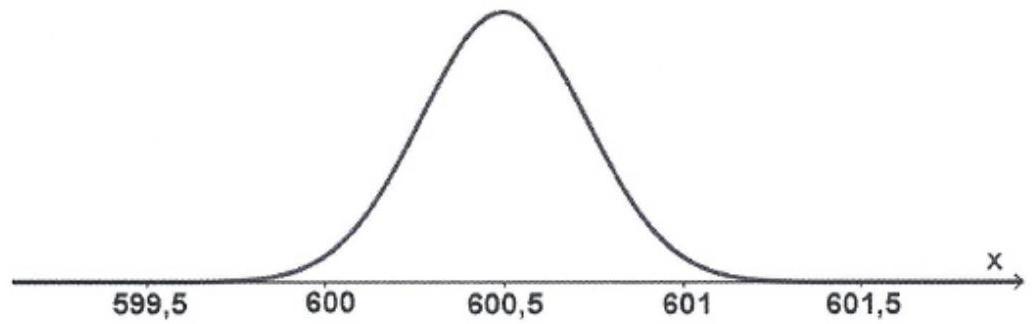
\includegraphics[max width=\textwidth, center]{2025_04_24_cc848bbd8106d0cae39fg-3}

Abbildung 2:\\
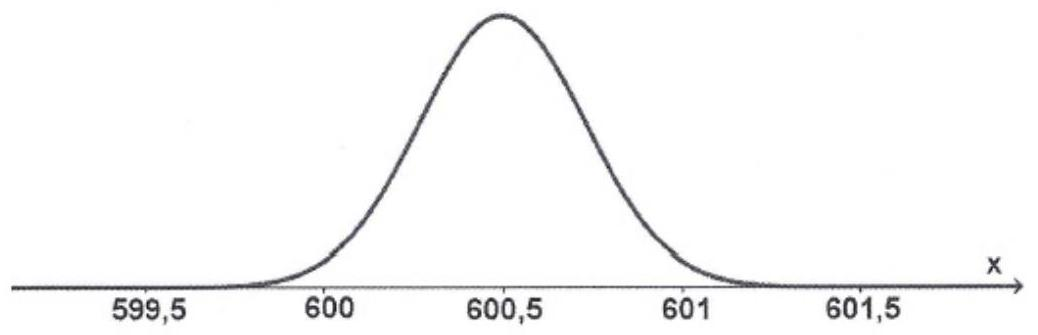
\includegraphics[max width=\textwidth, center]{2025_04_24_cc848bbd8106d0cae39fg-3(1)}

\section*{Lösungen}
\section*{Aufgabe C1}
a) Formulieren Sie eine passende Aufgabenstellung und erläutern Sie den Ansatz der Rechnung.

Die Wahrscheinlichkeit 0,985 bedeutet, dass eine Flasche mindestens 600 ml Ö। enthält.\\
Die Wahrscheinlichkeit $0,985^{12}$ bedeutet, dass in einem Karton mit 12 Flaschen jede Flasche mindestens 600 ml Öl enthält.\\
b) Ermitteln Sie, wie viele Flaschen mindestens geliefert werden.

Die Zufallsgröße X gibt die Anzahl der Flaschen an, die mindestens 600 ml Öl enthalten.\\
Laut Aufgabenstellung ist der Erwartungswert mehr als 780.\\
Die Erwartungswertformel lautet $\mu=\mathrm{n} \cdot \mathrm{p}$.\\
$\mathrm{n} \cdot 0,985>780 \Leftrightarrow \mathrm{n}>791,8$\\
Es werden mindestens 792 Flaschen geliefert.\\
c) Bestimmen Sie die Wahrscheinlichkeit dafür, dass mehr als 3\% der Kartons fehlerhaft sind.

Die Zufallsgröße X gibt die Anzahl der Flaschen an, die weniger als 600 ml Ö। enthalten.\\
X ist binomialverteilt mit $\mathrm{n}=12$ und $\mathrm{p}=0,015$.\\
$\mathrm{P}($, ,Karton ist fehlerhaft" $)=\mathrm{P}(\mathrm{X} \geq 2)=1-\mathrm{P}(\mathrm{X} \leq 1) \approx 0,0134$\\
Die Zufallsgröße Y gibt die Anzahl der fehlerhaften Kartons an.\\
$Y$ ist binomialverteilt mit $n=150$ und $p=P(X \geq 2) \approx 0,0134$\\
$P(Y \geq 0,03 \cdot 150)=P(Y \geq 5)=1-P(Y \leq 4) \approx 0,052$\\
Die gesuchte Wahrscheinlichkeit beträgt ca. 0,052.\\
d) Ermitteln Sie für die folgenden Ereignisse jeweils die Wahrscheinlichkeit:

A: „Die Flasche enthält mehr als 601 ml Öl."\\
B: „Die Füllmenge der Flasche weicht höchstens um 0,5 ml vom Erwartungswert ab."

Die Zufallsgröße X gibt die Füllmenge einer Flasche in ml an.\\
$X$ ist normalverteilt mit $\mu=600,5$ und $\sigma=0,23$.\\
$\mathrm{P}(\mathrm{A})=\mathrm{P}(\mathrm{X}>601) \approx 0,0149$\\
$\mathrm{P}(\mathrm{B})=\mathrm{P}(600 \leq \mathrm{X} \leq 601) \approx 0,970$\\
e) Begründen Sie, dass die Verwendung der Normalverteilung dennoch sinnvoll ist.

Die Wahrscheinlichkeit, die die verwendete Normalverteilung für negative Füllmengen liefert, ist so gering, dass sie im Sachzusammenhang vernachlässigt werden kann.\\
f) Skizzieren Sie in der Abbildung 1 den Graphen einer Dichtefunktion, die sich aus dem Vorschlag 1 ergeben könnte, und in der Abbildung 2 den Graphen einer Dichtefunktion, die zum Vorschlag 2 passt. Begründen Sie für jeden Vorschlag mithilfe des skizzierten Graphen, dass damit das Ziel des Unternehmens erreicht wird.

Abbildung 1:
Der bisherige Erwartungswert von 600,5 wird erhöht.\\
Das Schaubild der Dichtefunktion verschiebt sich dadurch nach rechts, da der xWert des Hochpunktes den Erwartungswert darstellt.\\
Der Vorschlag funktioniert, da die Fläche für $\mathrm{x} \leq 600$ zwischen der x -Achse und der gestrichelten Kurve kleiner wird.\\

Abbildung 2:
Wenn die Genauigkeit erhöht wird, verringert sich die Standardabweichung. Das Schaubild der Dichtefunktion wird damit um den Hochpunkt steiler, der y-Wert des Hochpunktes wird aber größer, da ansonsten die Fläche zwischen dem Schaubild und der x-Achse kleiner als 1 werden würde. Der Vorschlag funktioniert, da die Fläche für $\mathrm{x} \leq 600$ zwischen der x -Achse und der gestrichelten Kurve kleiner wird.\\

g) Ermitteln Sie den kleinsten möglichen Wert von n.

Die Wahrscheinlichkeit, dass bei $n$ Motiven $n$ Flaschen gezogen werden, die alle Motive unterschiedlich sind beträgt\\
$P=\frac{n}{n} \cdot \frac{n-1}{n} \cdot \frac{n-2}{n} \cdot \ldots \frac{1}{n}=\frac{n!}{n^{n}}$\\
Hinweis:\\
Bei der ersten Ziehung ist das Motiv egal, bei der zweiten Ziehung stehen noch n -1 Motive zur Wahl, bei der dritten Ziehung noch n-2 Motive usw.

Probe mit dem Taschenrechner:\\
$\mathrm{n}=6: \frac{6!}{6^{6}} \approx 0,0154>0,01$\\
$\mathrm{n}=7: \frac{7!}{7^{7}} \approx 0,006<0,01$\\
Der kleinste Wert ist $\mathrm{n}=7$.


\end{document}